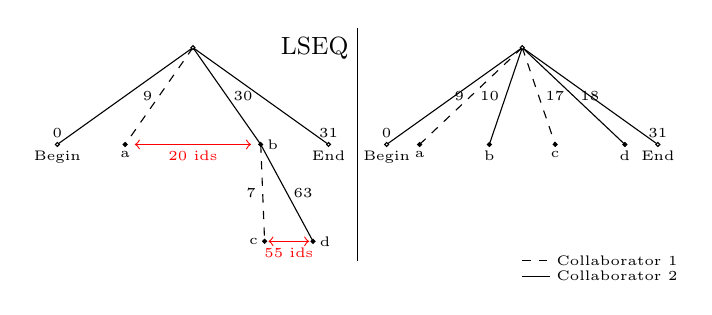
\begin{tikzpicture}[scale=0.7]
  \small

  \draw ( 85pt,10pt)node[anchor=north east]{LSEQ} node[anchor=north
  west]{\NAME{}}--( 85pt, -110pt);

  \tiny

  \draw (0,0) -- (-70pt, -50pt);
  \draw (0,0) -- ( 70pt, -50pt);

  \draw[dashed] (0,0) -- node[anchor=east]{9}  (-35pt, -50pt);
  \draw (0,0) -- node[anchor=west]{30} ( 35pt, -50pt);

  \draw[dashed] (35pt, -50pt) -- node[anchor=east]{7} (37pt, -100pt);
  \draw (35pt, -50pt) -- node[anchor=west]{63} (62pt, -100pt);

  \draw[fill=white] (0,0) circle (1pt);

  \draw[fill=white] (-70pt, -50pt) node[anchor=north]{Begin}
  node[anchor=south]{0} circle (1pt);

  \draw[fill=white] ( 70pt, -50pt) node[anchor=north]{End}
  node[anchor=south]{31} circle (1pt);

  \draw[fill=black] (-35pt, -50pt) node[anchor=north]{\ELEM{a}} circle (1pt);
  \draw[fill=black] ( 35pt, -50pt) node[anchor=west]{\ELEM{b}} circle (1pt);

  \filldraw[black] (37pt, -100pt) node[anchor=east]{\ELEM{c}} circle (1pt);
  \filldraw[black] (62pt, -100pt) node[anchor=west]{\ELEM{d}} circle (1pt);

  \draw[<->,color=red] (-30pt,-50pt) -- node[anchor=north]{20 ids}
  (30pt,-50pt);
  
  \draw[<->,color=red] (39pt,-100pt) -- node[anchor=north]{55 ids}
  (60pt,-100pt);

%% % % % %  %% %%% %% % % % % % %% % % % %%% %
  
  \draw (170pt,0pt) -- ( 100pt,-50pt);
  \draw (170pt,0pt) -- ( 240pt,-50pt);

  \draw[dashed] (170pt,0pt)--node[anchor=east]{9}(117pt,-50pt);
  \draw (170pt, 0pt)--node[anchor=east]{10}  (153pt,-50pt);
  \draw[dashed] (170pt, 0pt)-- node[anchor=west]{17} (187pt,-50pt);
  \draw (170pt, 0pt) --node[anchor=west]{18} (223pt,-50pt);

  \draw[fill=white] (170pt,0) circle (1pt);

  \draw[fill=white] (100pt,-50pt)node[anchor=north]{Begin}
  node[anchor=south]{0} circle(1pt);

  \draw[fill=white] (240pt,-50pt)node[anchor=north]{End}
  node[anchor=south]{31}circle(1pt);



  \draw[fill=black] (117pt,-50pt) node[anchor=north]{\ELEM{a}} circle (1pt);
  \draw[fill=black] (153pt,-50pt) node[anchor=north]{\ELEM{b}} circle (1pt);
  \draw[fill=black] (187pt,-50pt) node[anchor=north]{\ELEM{c}} circle (1pt);
  \draw[fill=black] (223pt,-50pt) node[anchor=north]{\ELEM{d}} circle (1pt);

  \begin{scope}[shift={(170pt,-110pt)}]
    \draw[dashed] (0,0) -- (0.5,0) node[right]{Collaborator 1};
    \draw[yshift=-\baselineskip-2pt] (0,0) -- (0.5,0) node[right]{Collaborator
      2};
  \end{scope}  

\end{tikzpicture}

%%% Local Variables: 
%%% mode: latex
%%% TeX-master: "../dchanges"
%%% End: 
